\chapter{Apéndice del Capítulo \ref{chapter:PO}}\label{app:PO}

%\section{Supporting information}
\section{Información de soporte}

\begin{figure}[htpb]
    \centering
    \hbox{\hspace{-2.5em}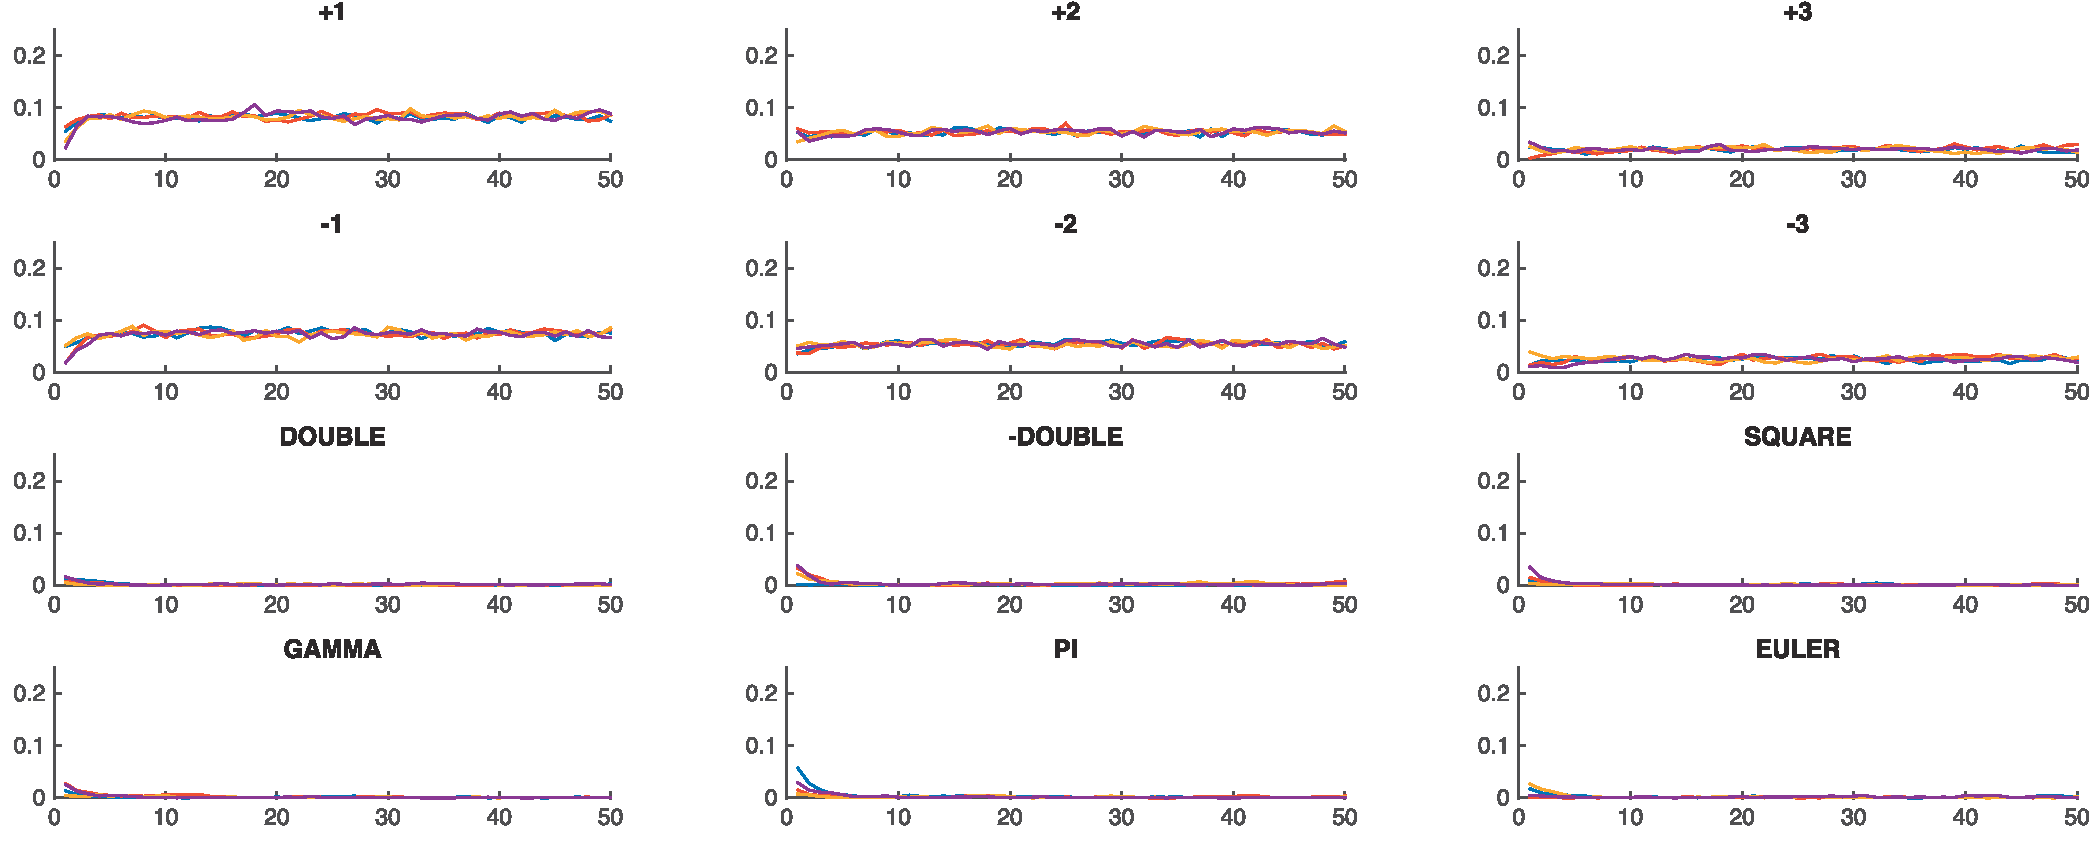
\includegraphics[width=1.2\textwidth]{figuras/plosone/S1Fig-eps-converted-to-a.pdf}}
    \hbox{\hspace{-2.5em}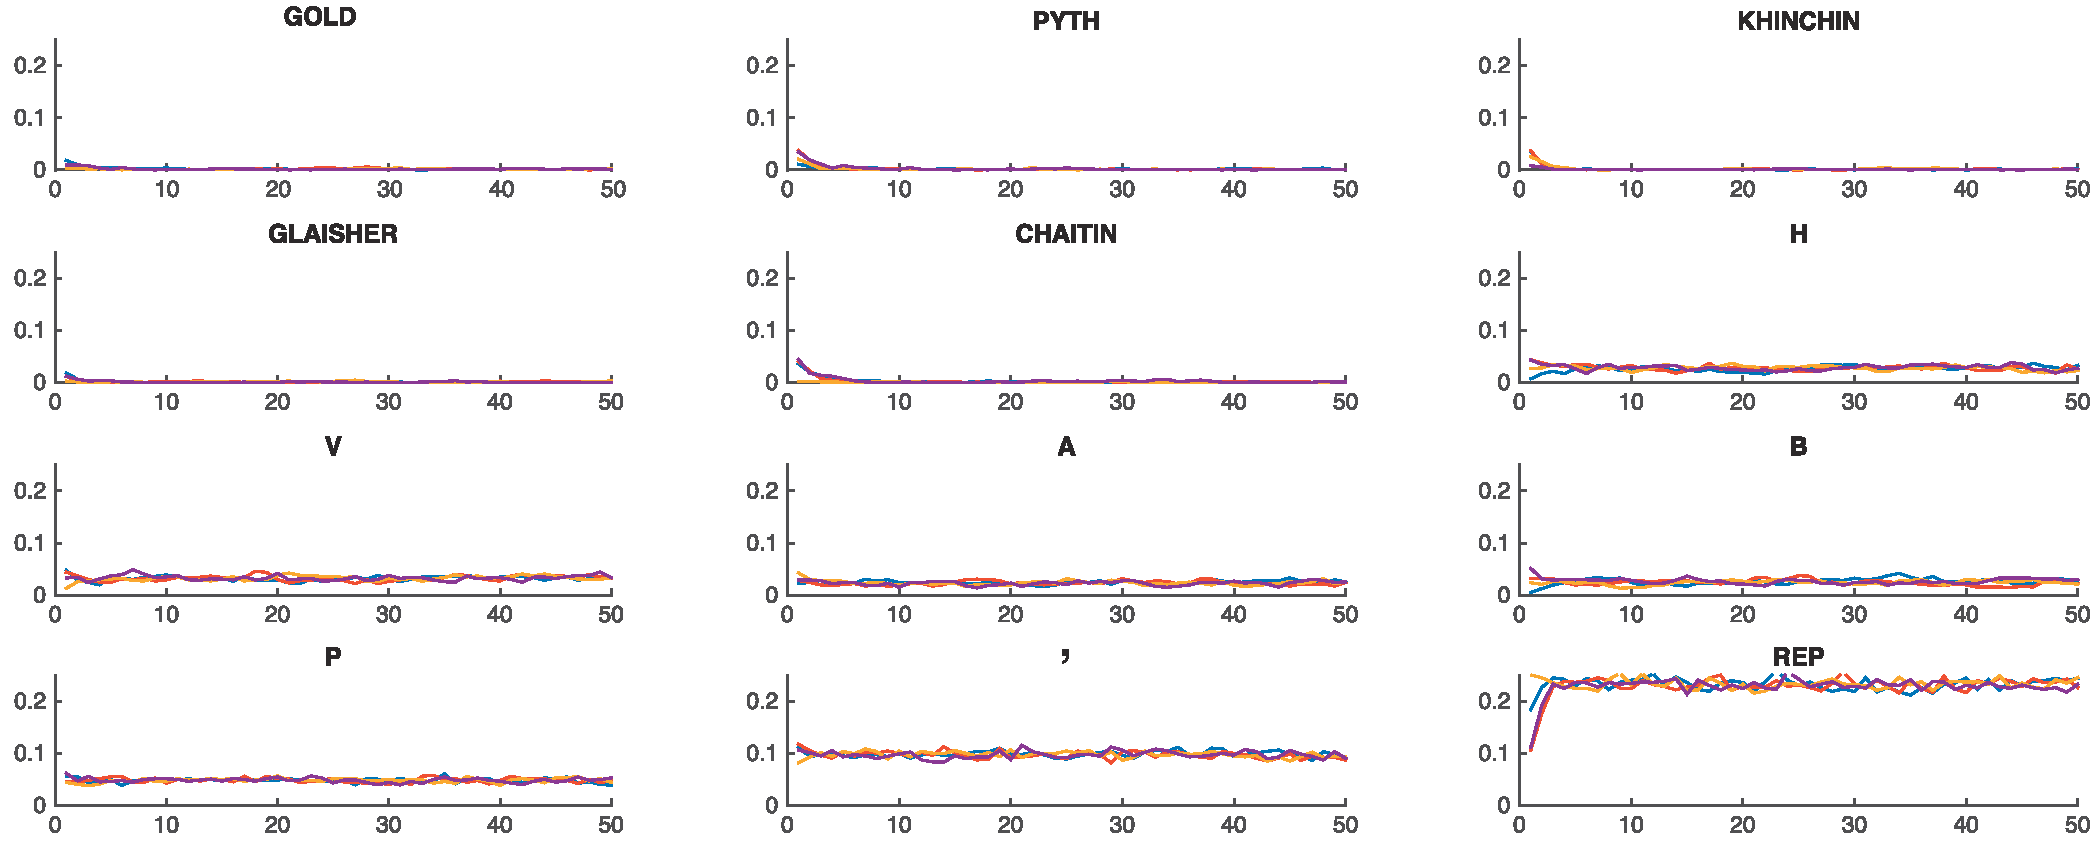
\includegraphics[width=1.2\textwidth]{figuras/plosone/S1Fig-eps-converted-to-b.pdf}}
    %\caption{\bf{MCMC steps for $\gramgeo$'s productions.} MCMC steps for the rest of $\gramgeo$'s grammar productions.}
    \caption{Pasos de MCMC para el resto de las producciones de la gramática $\gramgeo$.}
    \label{S1_Fig}
\end{figure}

\begin{figure}[htpb]
    \centering
    \hbox{\hspace{-2.5em}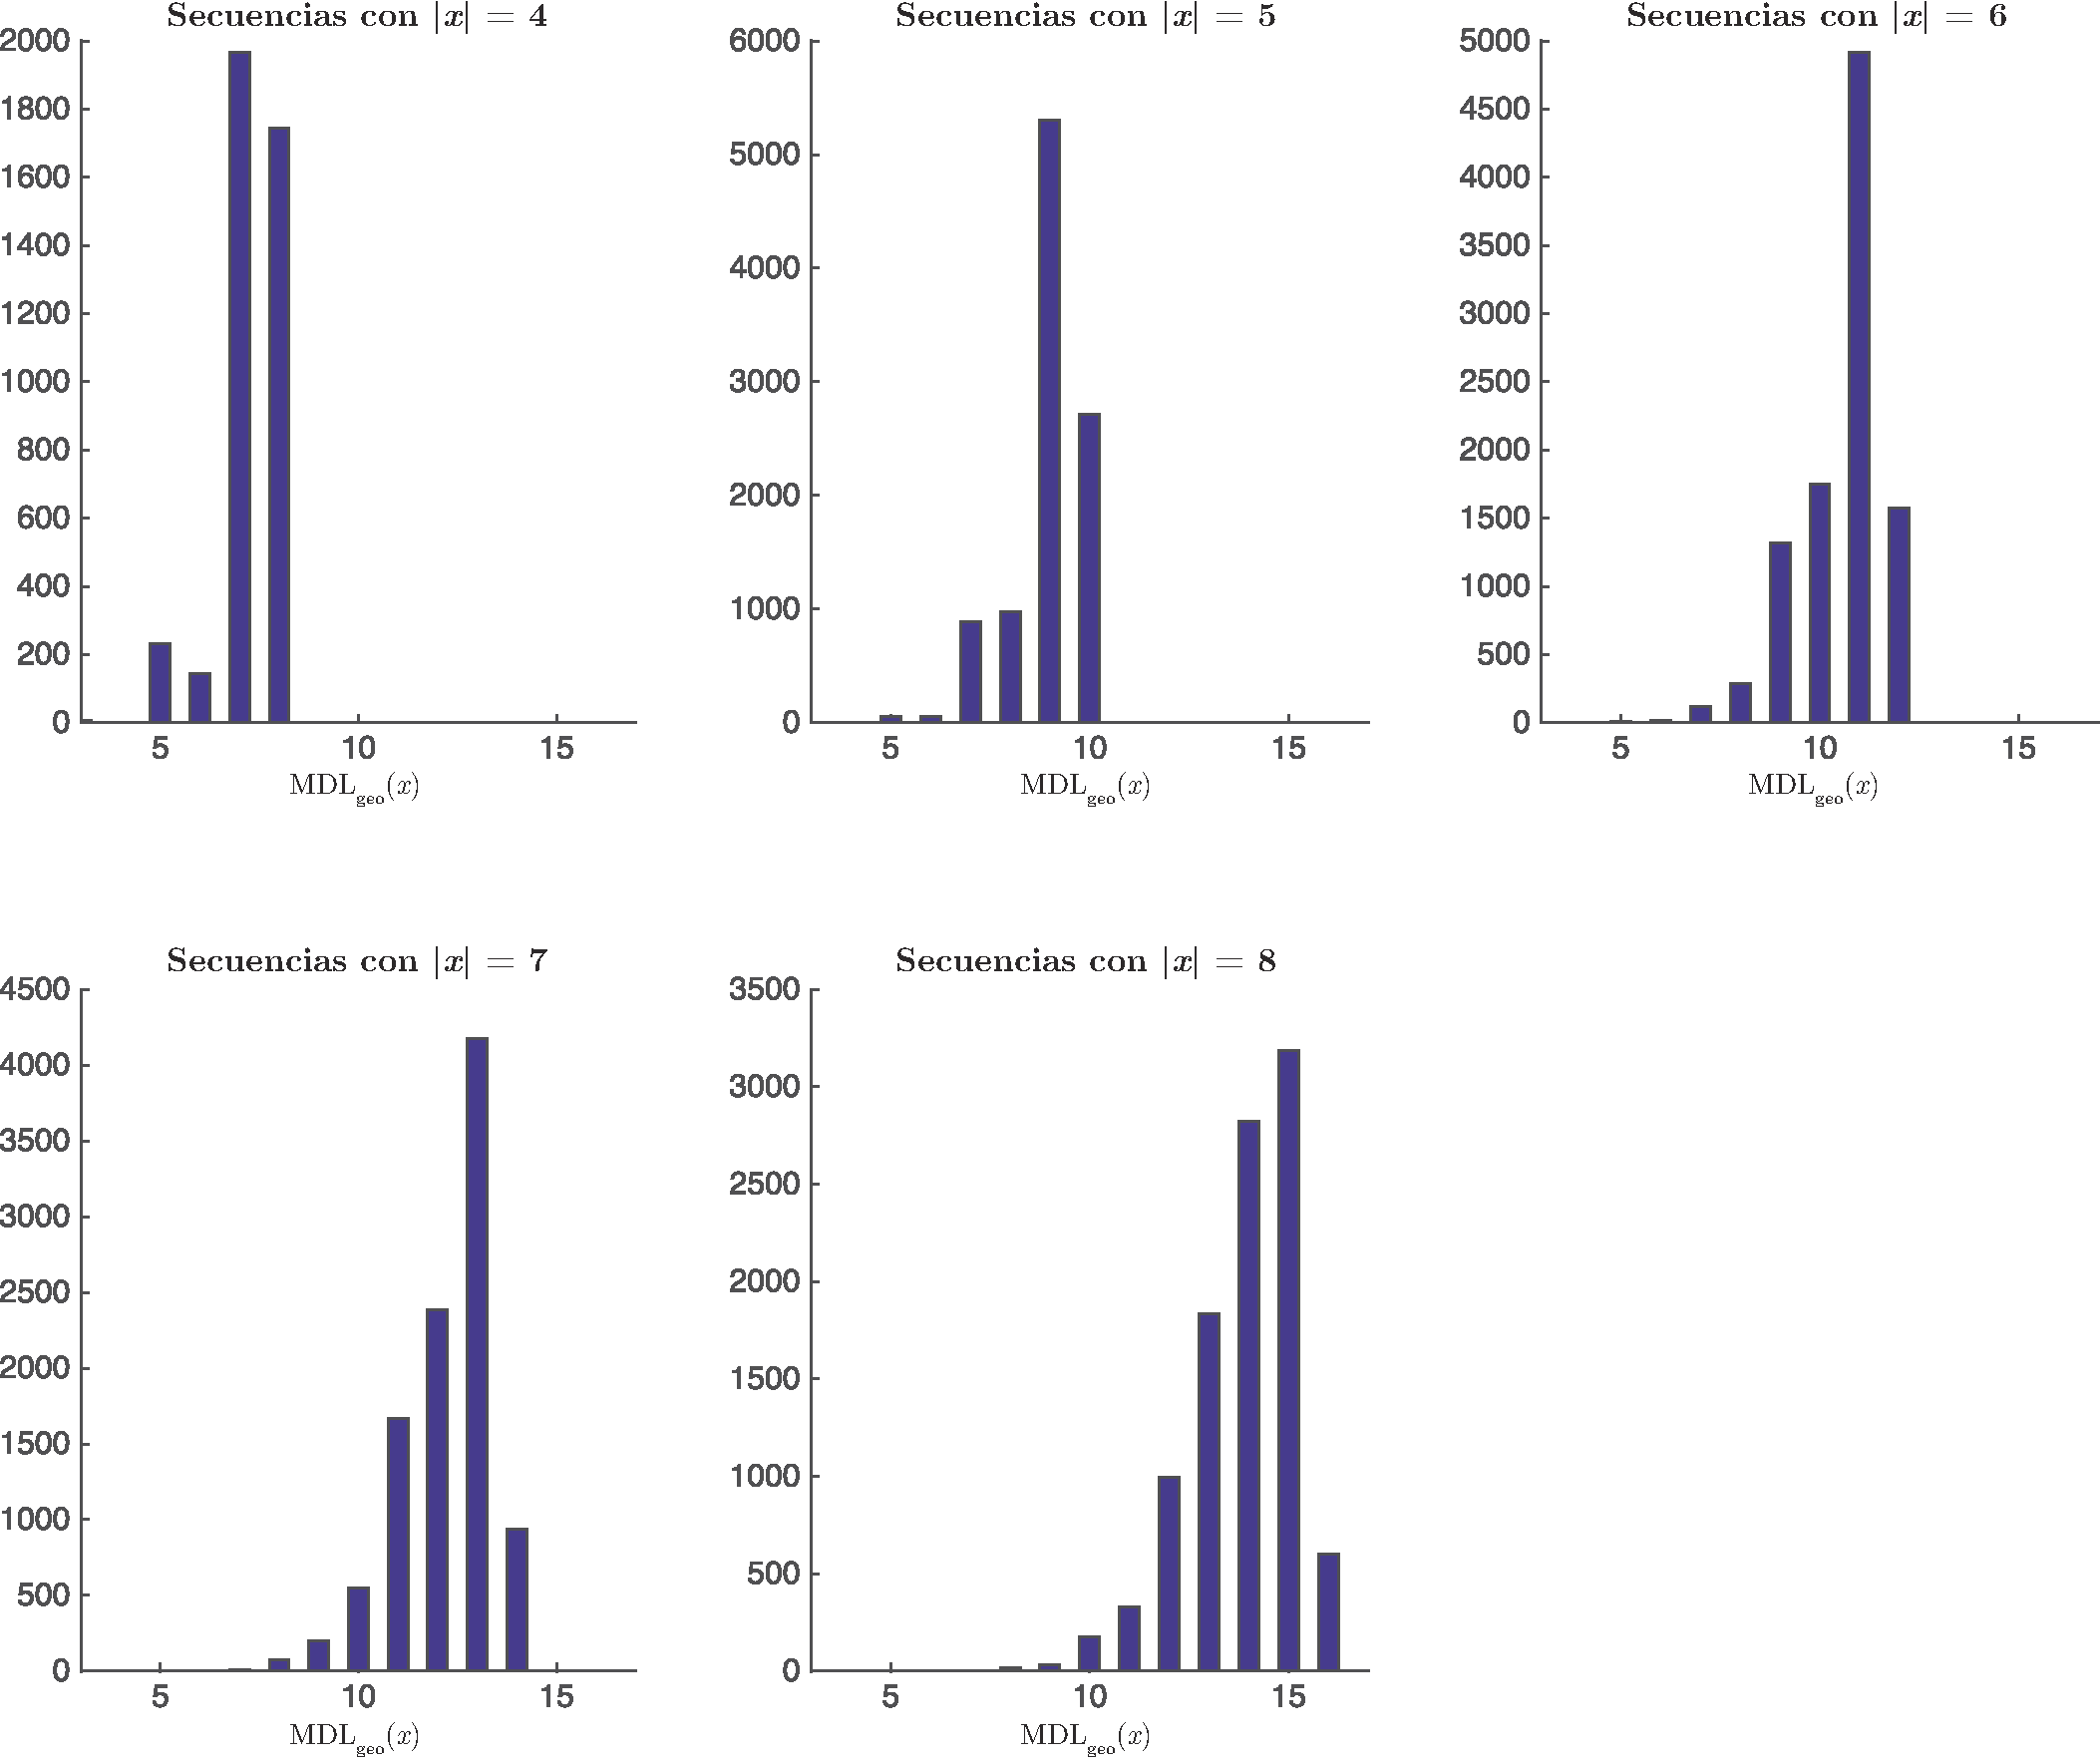
\includegraphics[width=1.2\textwidth]{S2Fig-eps-converted-to.pdf}}
    %\caption{\bf{Histograms of complexity $K_{\gramgeo}(x)$}. Histograms of  complexity for sequences with length between 4 and 8.}
    \caption{Histogramas de complejidad $\mdlgeo(x)$ para secuencias con longitud entre 4 y 8.}
    \label{S2_Fig}
\end{figure}

\begin{figure}[htpb]
    \centering
    \hbox{\hspace{-2.5em}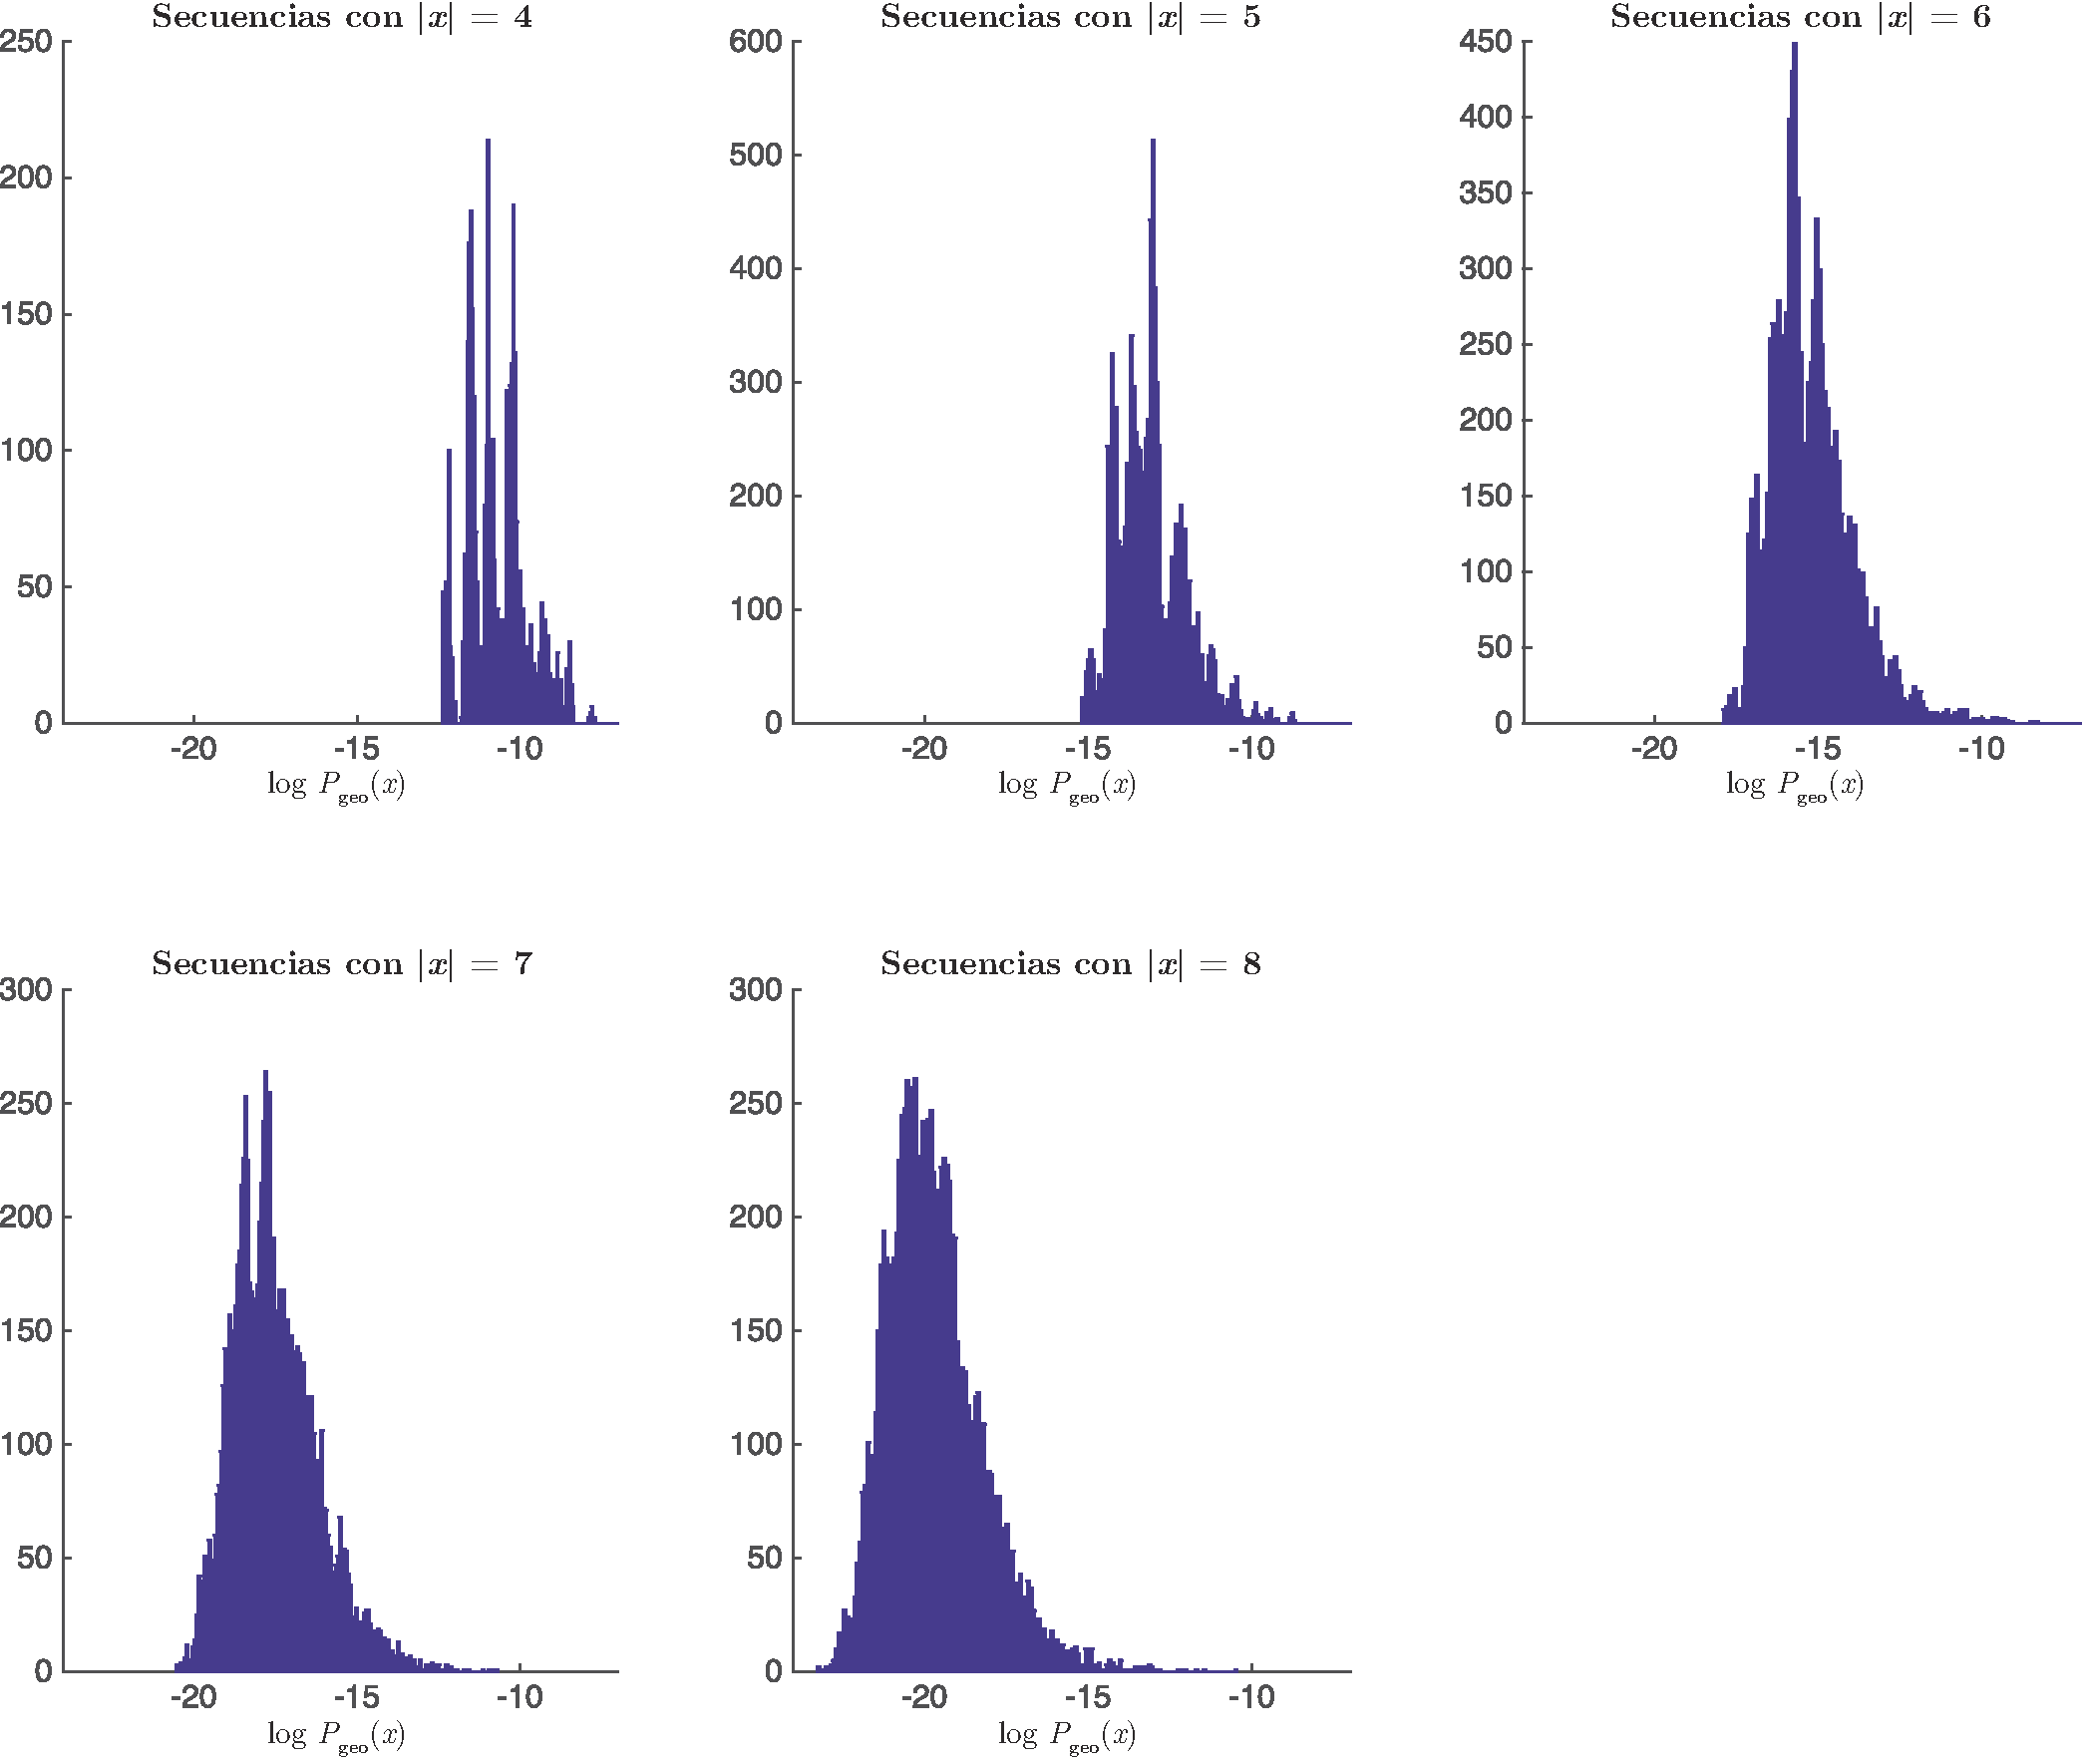
\includegraphics[width=1.2\textwidth]{S3Fig-eps-converted-to.pdf}}
    %\caption{\bf{Histograms of probability $P_{\gramgeo}(x)$}. Histograms of  probability for sequences with length between 4 and 8.}
    \caption{Histogramas de probabilidad $P_{\gramgeo}(x)$para secuencias con longitud entre 4 y 8.}
    \label{S3_Fig}
\end{figure}